% !TEX root =  ../Dissertation.tex

\chapter{Evaluation}
\section{Surveys and User Satisfaction}
The findings of this project are predominantly split into two. Findings from evaluating users and findings from the data tracking done on the website by Google Analytics. This section of the report will distil the findings of these two methodologies and what can be learned from the twenty users who used both applications, Wordle with no login and Wordle with increased features, to track how many more were retained from the increased features. 

Before users entered the experiment, an entrance survey was sent to gather information about their previous interactions with Wordle. The amount that people have played and still play varied greatly. The entrance survey clearly showed that most felt positive about adding more features and more of an ability to interact with friends and family. There was a clear consensus that adding the features suggested on the goals page was a great starting point to add more intractability to a daily game genre web app. 

In the exit survey, most users were satisfied with the gauntlet overall, with an average rating of 4.2/5. The leaderboard feature was the clear favourite for user satisfaction, achieving a rating of 4.73/5. From the comments, it is evident that it did elicit the hoped effect from users. 14/15 users said that the leaderboard encouraged them to play more, and 11/15 users mentioned the word "competition" or "competitiveness; the rest praised the feature for its social aspects.

Something else that became clear was that many users did not understand or enjoy the share feature, with it achieving a rating of 3.67/5. When checking the database, it was the least-used feature in the web application as it was only used for twelve different words over the seven days. Because of this, a question was added to the exit survey asking users if they understood what the share button did. 33 percent of people did not understand the feature and quite a few of the users who did were not in favour of it. What emerged from the exit form was that many people didn't explore the feature. One user commented that "there was no incentive to share". In hindsight, what could have been done for this is associating achievements with shared games; this would be similar to how Clash of Clans have incentives to invite other users to use the game, which would help with user acquisition. While the share feature was not a complete failure, some users still used and enjoyed it. It has become evident that there was not enough clarity as to what the share function did, and there was not much to be gained in using it. 

Achievements did well in satisfaction, not as well as leaderboards but not as poorly as shared. It ended with an average score of 4/5 from users. 27 percent of users said they were not encouraged to continue playing because of the achievements system. Originally when produced the main issue that was foreseen with achievements was the rudimentary nature of them. None of them were too in-depth and primarily based on how many wins and losses you achieved. What most users took issue with, however, was that there was no social aspect to them. One user mentioned, "I personally had no interest in obtaining achievements for the game. The ones I did get were mostly by luck/accidentally. It was not a negative to my experience. Perhaps if there were a leaderboard (or other way of comparing to others) for the achievements themselves this would be different (if there was, I didn't notice it).". Another user said, "I like when achievements are part of a bigger network like Steam or Xbox but they don't motivate me as a one-off.". From these comments, a change that could be made that would improve the achievement system could be the ability to compare your achievements to another user, similar to how you can on Steam, adding a level of sociability not yet found in the achievements system. 

\begin{figure}[h] % 'h' means 'here' - places the figure where it's defined
    \centering
    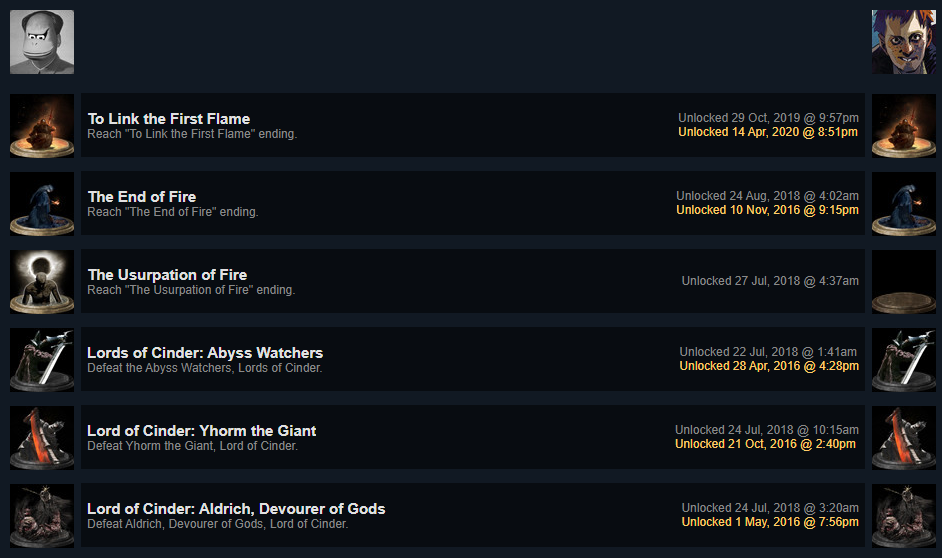
\includegraphics[width=\textwidth]{Steam_Achievements_Comparison.png} % Replace with your image file
    \caption{An example of comparing achievements on Steam}
    \label{fig:example}
\end{figure}

Wordle with increased word length also seemed to be a success for user satisfaction with 27 percent of players listing it as the number one feature that encouraged them to play more. One concern when developing this feature was that it would be too frustrating for users to play, as coming up with an eight-letter word is significantly harder than a five-letter word. In the exit survey, most commented that while it was fairly challenging, the users also felt more rewarded when they solved it. One user commented, "Increased word length up to 6 was challenging, but the number of eliminated letters per guess makes 7 and 8 letters quite easy". This was a surprise, but perhaps only one user commenting on this makes it a partial outlier in the game's believed increased difficulty. 

\section{Data Analytics}
All users had access to both websites and were prompted to use them as much as they pleased for a week. Google Analytics was set up for both websites to compare how many users remained using both websites. This allows other valuable information to be gleaned from the analytics that Google provides. 

As expected, Wordle had no features, and The Gauntlet had roughly the same number of users, with the Gauntlet at 34 and Wordle at 33 over the seven days. While the website was only sent to twenty people, it's apparent that some users sent the website to others, so it is not unexpected that there are a few more users. Interestingly, on the first day of the experiment, two more users used Wordle over the Gauntlet. 

\begin{figure}[h] % 'h' means 'here' - places the figure where it's defined
    \centering
    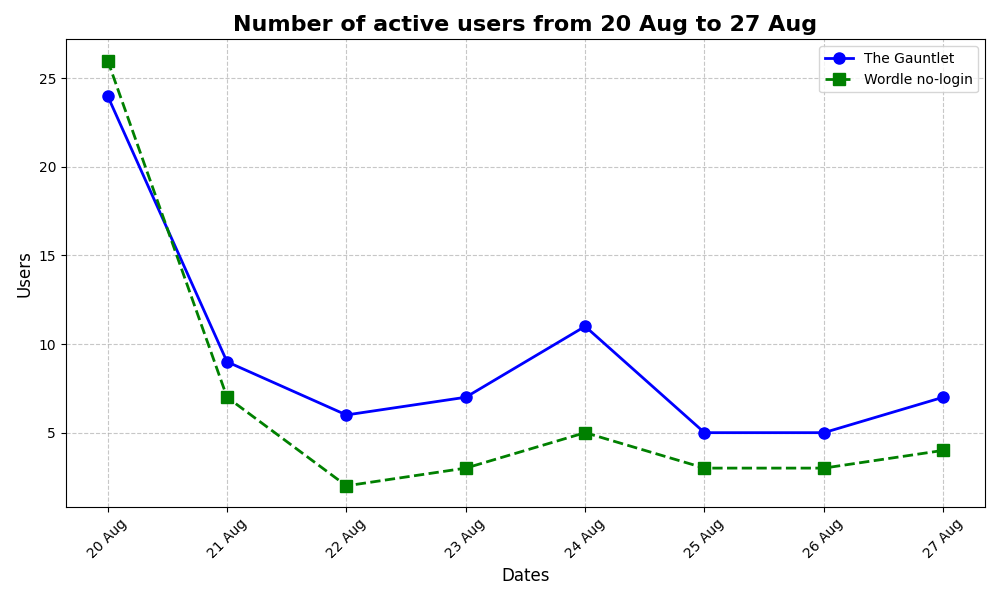
\includegraphics[width=\textwidth]{Number of Active Users Gauntlet.png} % Replace with your image file
    \caption{Graph of active users during the experiment on both web apps}
    \label{fig:example}
\end{figure}

After the first day, usage sharply declines. This is expected with games such as this, as shown by Mistplay, a company that focuses on a loyalty reward system for gamers using its suite of games. Mistplay released an article showing the retention rates of its games, and even on the first day, it retains only 30 percent of the users who try the application\cite{mistplay2024}. On the third day, The Gauntlet's user numbers stabilised, maintaining a user base of five to seven users daily, with an uptick on Saturday to eleven users. Wordle, by comparison, on the third day, had stabilised to a user base of two to four, with an uptick on Saturday of a user base of five. These increases during the weekend are likely due to users playing more games on a weekend rather than a weekday (Cite article here). From this data, it is apparent that the users have tended more to use The Gauntlet over Wordle with no login in terms of active users each day.

Another aspect in which The Gauntlet has outperformed Wordle with no login web app is user engagement. Over the seven days that the experiment lasted, Wordle, with no login, had an average engagement time of 1 minute and 44 seconds. Conversely, The Gauntlet had an average engagement time of 10 minutes and 54 seconds. A part of this increase can likely be accredited to users having to spend longer to solve a longer. Also, users will be more likely to play multiple games in a single session to improve their leaderboard rating or attempt to attain an achievement. 

\begin{figure}[h] % 'h' means 'here' - places the figure where it's defined
    \centering
    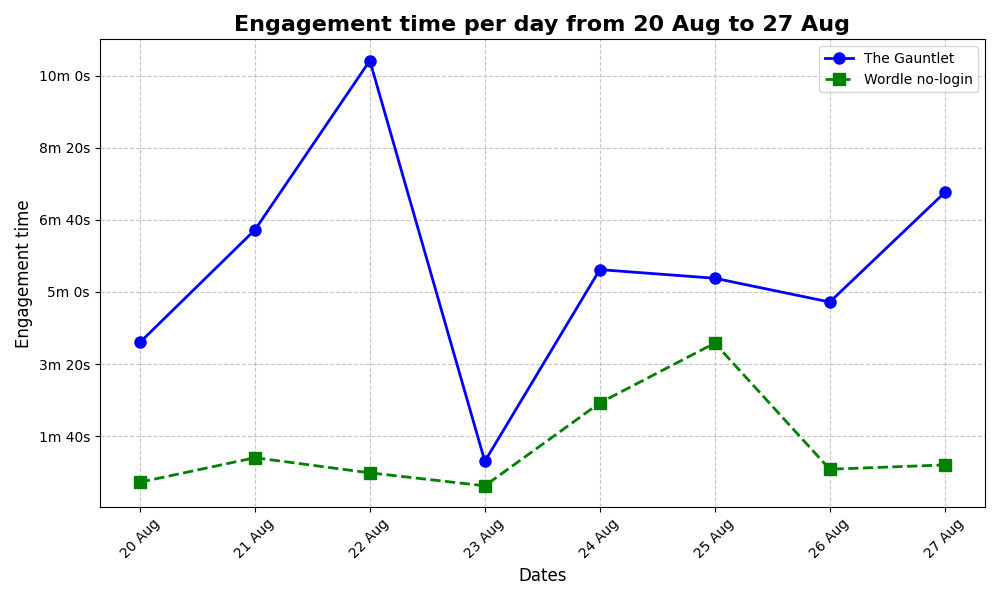
\includegraphics[width=\textwidth]{Engagement_Time.png} % Replace with your image file
    \caption{Average Engagement time each day for both web apps}
    \label{fig:example}
\end{figure}

\clearpage

Google Analytics also tracks the number of "events" triggered on a website. An "event" occurs whenever a user interacts with the website in any way, whether they change pages, make a guess, or change the website's state. Throughout the experiment, Google Analytics tracked 304 events on the Wordle without login, while The Gauntlet had 1500. It should be pointed out that this may not be the strongest comparison between the two websites, as The Gauntlet has many more events to trigger over Wordle with no login. Looking at the database for overall games, 191 games were played on The Gauntlet, while only 40 games were played on Wordle with no login. 

\begin{figure}[h] % 'h' means 'here' - places the figure where it's defined
    \centering
    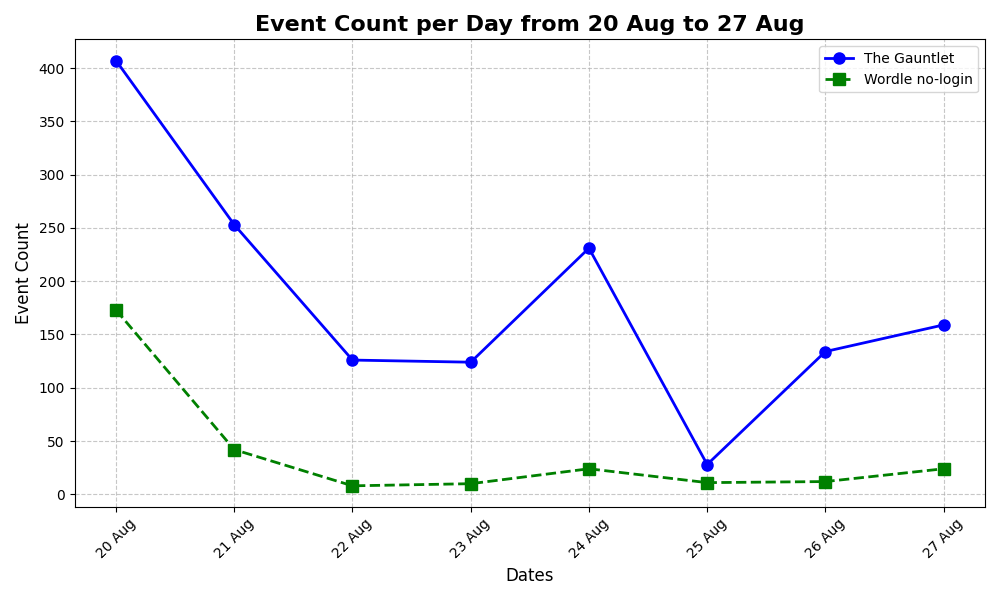
\includegraphics[width=\textwidth]{Event_count_per_day.png} % Replace with your image file
    \caption{Event Count each day for both web apps}
    \label{fig:example}
\end{figure}

Overall, it is clear that The Gauntlet has better metrics in every aspect compared to Wordle with no login. While it is hard to show in the data what aspects of The Gauntlet increased user retention the most, a general idea can be formed by the user satisfaction as user satisfaction is shown to be a direct indicator of user retention in features (Cite StumbleUpon article). The share feature seems to have had little effect due to unclear signposting of what the feature did and users not thinking it added much value to the overall web app, while leaderboards seem to be the retention technique with the greatest effect, achievements also being a valuable addition to retention.
\clearpage
\section{Requirements Met}
Now that The Gauntlet has been tested and evaluated by users and data metrics, it's pertinent that the functional and non-functional requirements are checked to see if it has reached its desired state. Most requirements are met, so this section will look at those that weren't.

\begin{figure}[h] % 'h' means 'here' - places the figure where it's defined
    \centering
    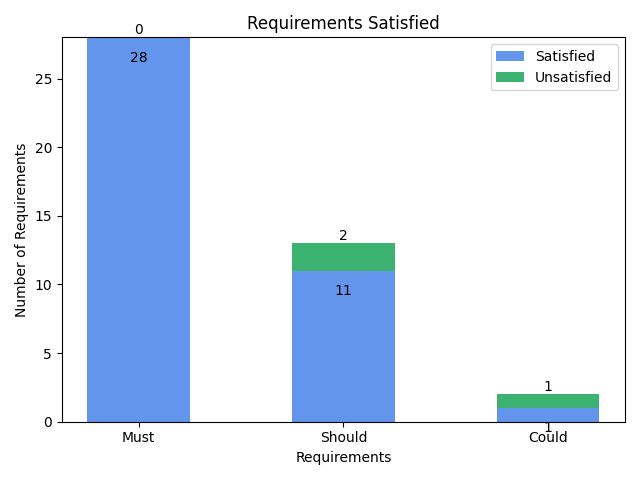
\includegraphics[width=\textwidth]{Requirements_Met.png} % Replace with your image file
    \caption{Graph of requirements met.}
    \label{fig:example}
\end{figure}


\begin{itemize}[leftmargin=*, label=\textbullet]
    \item \textbf{Have an option to suggest achievements} This was originally conceptualised as an offering so that users could suggest achievements in a submission box to better understand how the achievement section could be improved. When prototyping this component, it harmed the aesthetics of the achievements page greatly for something no longer believed to add too much value to the project, as users were generally messaging the developer personally to suggest changes about all aspects of the website. In the future, something like this could be added as a separate page to invite suggestions on changes to any part of the website, as personal messages about improving the site to the developer directly are not scalable enough to consider all users' opinions.

    \item \textbf{Layout should match the qwerty layout} This functional requirement was only attempted later in development when dealing with fixes and smaller additions. When attempting to add this requirement, it created large issues on the phone version of the web application where the keyboard would take up an amount of the screen, which meant users could not fully see the game they were playing. In future works, it should be possible to achieve this requirement, and this functionality was just left unfixed due to time constraints.

    \item \textbf{Have guesses be checked against a comprehensive English dictionary}
    During the development of the web application, many different large libraries of English words were used to check that users' words were valid guesses for Wordle. The issue that was raised by users when they eventually started using the web application was that these libraries invalidated words that should be validated. Eventually, this feature was scrapped to prevent users from being frustrated with invalid guesses. There must be a library large enough to fix this issue, but one that had open access was not found during development. 


\end{itemize}